\documentclass[a4paper,11pt,headsepline]{report} % scrreprt würde auch gehen

\usepackage{titling}

%----------------- PDF CONFIG ----------------- %
\pdfinfo{    
     /Title     (Masterthesis  ++Davidoff Robert++ - HSRM WI - ++Entwicklung eines dezentralen Identitätsmanagementsystems basierend auf Distributed Ledger Technology (DLT)++) 
     /Subject   (Masterthesis  ++Davidoff Robert++)    
     /Author    (++Davidoff Robert++) 
     /Keywords  (Master,Masterthesis,HSRM)      
} 

\title{Entwicklung eines dezentralen Identitätsmanagementsystems basierend auf Distributed Ledger Technology (DLT)}
\author{Davidoff Robert}
\date{++AbgabeDatum++}



%----------------- PAKETE INKLUDIEREN ----------------- %

\usepackage[enable]{easy-todo} % Bietet eine art TODO Liste an; Zum bauen des abgabebereiten Dokumentes sollte die Option enable durch disable ersetzt werden!

\usepackage{geometry} % Packet für Seitenrandabständex und Einstellung für Seitenränder
\usepackage[ngerman]{babel} % deutsche Silbentrennung
\usepackage{blindtext} % Für den Beispieltext
\usepackage{comment}
\usepackage{lscape}
\usepackage{colortbl}
\usepackage{amsfonts}

\usepackage{booktabs} % entzerrt die Tabellenzeilen und bietet verschieden dicke Unterteilungslinien
\usepackage{longtable} % Tabellen können sich nicht über mehrere Seiten 
\usepackage{graphicx} % kann LaTeX Grafiken einbinden
%\usepackage{parskip}
\usepackage{xstring} % Für das FakeSmallCaps

\usepackage[utf8]{inputenc}
%\usepackage[applemac]{inputenc} % Umlaute unter Mac werden automatisch gesetzt
\usepackage[T1]{fontenc} % Zeichenencoding
\usepackage{lmodern} % bessere typographische Qualität 
\frenchspacing % Schaltet den zusätzlichen Zwischenraum ab; Wird mit ngerman-babel schon geladen
\usepackage{fix-cm}
\usepackage{hyperref} % verwandelt alle Kapitelüberschriften, Verweise aufs Literaturverzeichnis und andere Querverweise in PDF-Hyperlinks
\usepackage{color}
\usepackage[table]{xcolor}
\usepackage{enumitem}
\usepackage{url}
\usepackage{acronym}
\usepackage[ddmmyyyy,hhmmss]{datetime}
\renewcommand{\dateseparator}{.}

\usepackage{tabu} % Tabellen nutzen
\usepackage{multirow}
\usepackage{booktabs}
\usepackage{setspace} % to use \singlespacing\onehalfspacing\doublespacing
\usepackage{mathtools}
\usepackage{float}
\usepackage{rotating} % For sidewayfigures
\usepackage{caption} % For centering the Captions if more than one Line
\captionsetup{justification=centering,margin=3em} % Set centering for captions as default

%----------------- SCHRFITEN ----------------- %
%\usepackage{bera} % Font package
%\usepackage{inconsolata} % MONOSPACE Font
%\usepackage{newcent}
\usepackage{charter} % modernere Serifen Font


\usepackage[nottoc]{tocbibind}

%----------------- BibLaTeX ----------------- %
\usepackage[
backend=bibtex,
style=alphabetic
]{biblatex}
\bibliography{literatur}

%\usepackage{filecontents}
%\usepackage{multibib}
%\newcites{supp}{Supplementary References}
%----------------- EPIGRAPH ----------------- %
\usepackage{epigraph}
\setlength{\epigraphwidth}{0.7\textwidth} % Epigraph ist 70% der Textbreite breit
% Mache epigraph in Sans-Serif
\let\oldepigraph\epigraph % Gegen Rekursion
\renewcommand{\epigraph}[2]{\oldepigraph{\textsf{#1}}{\textsf{#2}}}

% für zweispaltige Inhalsverzeichnisse
% http://texblog.org/2013/08/14/tidy-and-compact-table-of-contents-with-multitoc/
% \usepackage[toc]{multitoc}
% \renewcommand*{\multicolumntoc}{2} % Spaltenanzahl; default 2
% \setlength{\columnseprule}{0.5pt} % Columnseperatingline


%----------------- LISTINGS ----------------- %
\usepackage{listings}

% LSTCOLORS
\definecolor{background}{HTML}{F1F1F1}
\definecolor{lavender}{rgb}{0.9, 0.9, 0.98}

% Genrell Settings
\lstset{
  captionpos              = b,
  basicstyle              = \footnotesize\ttfamily,
%  backgroundcolor         = \color{background},
  numbers                 = left,
  numberstyle             = \scriptsize\color{background!70!black},
  stepnumber              = 1,
  numbersep               = 3ex,
  showstringspaces        = false,
  breaklines              = true,
  framesep                = 1ex,
  frame                   = l,%trb,
  framerule               = .35ex,
  xleftmargin             = 1.37ex,
%  frameround              = tttt,
  rulecolor               = \color{black},
  commentstyle            = \color{darkgray!80},
  escapeinside            = {<@[}{]@>}, % You can Escape inside the LST with <@[ ESCAPED_TEXT ]@>
  lineskip                = {-1.2pt},
  aboveskip               = {2em},
  belowskip               = {1em},
}

% PHP
\definecolor{dkgreen}{rgb}{0,.6,0}
\definecolor{dkblue}{rgb}{0,0,.6}
\definecolor{dkyellow}{cmyk}{0,0,.8,.3}
\definecolor{dkorange}{rgb}{1.0, 0.5, 0.0}

\lstset{
  language         = PHP,
  keywordstyle     = \color{dkblue},
  stringstyle      = \color{red},
  identifierstyle  = \color{dkgreen},
  emph             = [1]{php},
  emphstyle        = [1]\color{black},
  emph             = [2]{if,and,or,else,null,NULL},
  emphstyle        = [2]\color{dkorange},
  emph             = [3]{class,implements,namespace,public,private,protected,function,return,new,throw,try,catch,as,instanceof},
  emphstyle        = [3]\color{dkblue},
  morekeywords     = {class,implements,namespace,public,private,protected,function,return,new,throw,try,catch,as,instanceof},
}


% JSON  
\colorlet{punct}{red!60!black}
\definecolor{delim}{RGB}{20,105,176}
\colorlet{numb}{magenta!60!black}

\lstdefinelanguage{json}{
%  stringstyle      = \color{orange},
%  morestring       = [b]",
  literate         =
   *{0}{{{\color{dkgreen}0}}}{1}
    {1}{{{\color{dkgreen}1}}}{1}
    {2}{{{\color{dkgreen}2}}}{1}
    {3}{{{\color{dkgreen}3}}}{1}
    {4}{{{\color{dkgreen}4}}}{1}
    {5}{{{\color{dkgreen}5}}}{1}
    {6}{{{\color{dkgreen}6}}}{1}
    {7}{{{\color{dkgreen}7}}}{1}
    {8}{{{\color{dkgreen}8}}}{1}
    {9}{{{\color{dkgreen}9}}}{1}
    {:}{{{\color{punct}{:}}}}{1}
    {,}{{{\color{punct}{,}}}}{1}
    {\{}{{{\color{delim}{\{}}}}{1}
    {\}}{{{\color{delim}{\}}}}}{1}
    {[}{{{\color{delim}{[}}}}{1}
    {]}{{{\color{delim}{]}}}}{1}
    {"}{{{\color{red}{"}}}}{1}, % make " red
}

\lstdefinelanguage{yaml}{
  keywords        = {true,false,null},
  comment         = [l]{\#},
  morecomment     = [s]{/*}{*/},
  morestring      = [b]',
  morestring      = [b]",
}

\definecolor{lightgray}{rgb}{.9,.9,.9}
\definecolor{darkgray}{rgb}{.4,.4,.4}
\definecolor{purple}{rgb}{0.65, 0.12, 0.82}

\lstdefinelanguage{JavaScript}{
	keywords={typeof, new, true, false, catch, function, return, null, catch, switch, var, if, in, while, do, else, case, break},
	keywordstyle=\color{blue}\bfseries,
	ndkeywords={class, export, boolean, throw, implements, import, this},
	ndkeywordstyle=\color{darkgray}\bfseries,
	identifierstyle=\color{black},
	sensitive=false,
	comment=[l]{//},
	morecomment=[s]{/*}{*/},
	commentstyle=\color{purple}\ttfamily,
	stringstyle=\color{red}\ttfamily,
	morestring=[b]',
	morestring=[b]"
}

\lstset{
	language=JavaScript,
	backgroundcolor=\color{lightgray},
	extendedchars=true,
	basicstyle=\footnotesize\ttfamily,
	showstringspaces=false,
	showspaces=false,
	numbers=left,
	numberstyle=\footnotesize,
	numbersep=9pt,
	tabsize=2,
	breaklines=true,
	showtabs=false,
	captionpos=b
}

%----------------- FARBEN DEFINIEREN ----------------- %
% ~Hochschulfarben~
% Primary Colors
\definecolor{hsrmRed}{rgb}{0.882352941,0,0.098039216}
\definecolor{hsrmRedDark}{rgb}{0.588235294,0,0.058823529}
\definecolor{hsrmWarmGreyDark}{rgb}{0.274509804,0.254901961,0.235294118}
\definecolor{hsrmWarmGreyLight}{rgb}{0.666666667,0.647058824,0.62745098}

% Secondary Colors
\definecolor{hsrmSec1}{rgb}{0,0.588235294,0.509803922}
\definecolor{hsrmSec1Dark}{rgb}{0,0.392156863,0.31372549}
\definecolor{hsrmSec1Comp}{rgb}{0.294117647,0.745098039,0.882352941}
\definecolor{hsrmSec1CompDark}{rgb}{0.196078431,0.490196078,0.568627451}

\definecolor{hsrmSec2}{rgb}{0.607843137,0.764705882,0.156862745}
\definecolor{hsrmSec2Dark}{rgb}{0.411764706,0.490196078,0.098039216}
\definecolor{hsrmSec2Comp}{rgb}{0.254901961,0.156862745,0.509803922}
\definecolor{hsrmSec2CompDark}{rgb}{0.176470588,0.098039216,0.333333333}

\definecolor{hsrmSec3}{rgb}{0.509803922,0.078431373,0.31372549}
\definecolor{hsrmSec3Dark}{rgb}{0.338345865,0.058823529,0.196078431}
\definecolor{hsrmSec3Comp}{rgb}{1,0.509803922,0}
\definecolor{hsrmSec3CompDark}{rgb}{0.666666667,0.333333333,0}

% Custom Colors
\definecolor{gray}{gray}{0.95} % Listingsbackground
\colorlet{darkgray-light}{darkgray!90}

% Farbskala - um zB Prioritäten darzustellen
\definecolor{colorscale-green}{HTML}{DBFF33}
\definecolor{colorscale-yellow}{HTML}{FFF033}
\definecolor{colorscale-orange}{HTML}{FFBD33}
\definecolor{colorscale-dkorange}{HTML}{FF8A33}
\definecolor{colorscale-red}{HTML}{FF5733}
\definecolor{colorscale-gray}{gray}{.75}

%----------------- NEW Commands ----------------- %
% Eigener kurzer LoremIpsumDummyText
\newcommand{\sblindtext}{Dies hier ist ein Blindtext zum Testen von Textausgaben. Wer diesen Text liest, ist selbst schuld. Der Text gibt lediglich den Grauwert der Schrift an. Ist das wirklich so? Ist es gleichg\"{u}ltig, ob ich schreibe: ``Dies ist ein Blindtext'' oder ``Huardest gefburn''? Kjift $-$ mitnichten!}

% Define conclusionbox
\newcommand{\conclusionbox}[1]{\begin{center}\colorbox{darkgray!20}{\parbox{.9\textwidth}{#1}}\end{center}}

% Chapter Summary
\newcommand{\chaptersummary}[1]{\vspace{2em}\colorbox{darkgray-light}{\hspace{.03\textwidth}%
\parbox{.94\textwidth}{\vspace{.25em}%
\setlength{\parskip}{1.2ex}\bfseries\color{white}%
#1\vspace{1em}}%
\hspace{.03\textwidth}}%
\vspace{2em}}

% Fake Small Caps
\newcommand{\fakesmallcaps}[1]{\StrLeft{#1}{1} {\scriptsize\uppercase{\StrGobbleLeft{#1}{1}}}}

% Trenner
\newcommand{\trenner}{\centerline{\textcolor{risk-gray}{\rule{0.7\textwidth}{.4pt}}}}

% Table Midrule
\newcommand{\customcmidrule}[2]{\arrayrulecolor{#2}\cmidrule(l{1.5em} r{1.5em}){#1}\arrayrulecolor{black}}

% My Quote
\newenvironment{customquote}{\begin{quote}\raisebox{-.4\height}{{\Huge\color{darkgray-light} ''}}}{\end{quote}}



%----------------- LAYOUT SETZEN ----------------- %
\geometry{left=4.5cm, right=2cm, top=2.5cm, bottom=2.5cm}
\linespread {1.25}\selectfont %1.25 da er von Haus aus 1.2 ist und 1,25 * 1,2 = 1,5 isch
\setlength{\parindent}{0em} % im Deutschen Einrückung nicht üblich, leider
\setlength{\parskip}{1.2ex} % Abstand zum nächsten Absatz; evtl. KOMA verwenden?

%---------------- HEADER FOOTER ----------------------%
\usepackage{fancyhdr}
\pagestyle{fancy}
\newcommand{\phv}{\fontfamily{phv}\fontseries{m}\fontsize{9}{11}\selectfont}
%\addtolength{\headheight}{5ex} % damit man zwei Zeilen gut unterbringt
%\fancyhf{} % ClearFooter and Header
\fancyhead[LO,LE]{\small\selectfont\nouppercase\leftmark} % No uppercase and smaller fontsize
\fancyhead[RO,RE]{\small\selectfont\nouppercase\rightmark} % No uppercase and smaller fontsize
\lfoot{\phv \raisebox{-.24\height}{
\includegraphics[height=2.5ex]{media/logo_hsrm_single_bw}}\, Robert \textsc{Davidoff}} % \, ist ein kleiner Abstand
\cfoot{\thepage}




%-------##-------##-------##------- ANFANG INHALT -------##-------##-------##-------%
\begin{document}
\addtocontents{toc}{\protect\thispagestyle{empty}} % No Pagenumber on TOC Pages


\pagenumbering{roman} % Seitennummer

%----------------- DECKBLATT -----------------%
%----------------- KONFIGURATION -----------------%
\pagestyle{empty} % enthalten keinerlei Kopf oder Fuß

\newgeometry{left=4cm, right=2cm, top=1cm, bottom=1cm} % Mehr Platz oben und unten
%----------------- HS RM Logo -----------------%
\begin{figure}[t]
	\flushright
	
\includegraphics[width=0.3\textwidth]{media/logo_hsrm}
\end{figure}

%----------------- INHALT -----------------%

\begin{center}
Hochschule RheinMain \\
Fachbereich DCSM \\
Studiengang Master of Science - Informatik

% Whitespace
\vspace{30 pt}

{\Large \textbf{Masterthesis}} \\
zur Erlangung des akademischen Grades \\ 
Master of Science - M.Sc.\todoi{Stimmt der Grad?}

% Whitespace
\vspace{50 pt}

\begin{spacing}{1.2}
\LARGE \textbf{\thetitle}
\end{spacing}
%
\end{center}

\vfill % Fills all the space, so the follwing stuff is floating down

%
\begin{small}
\begin{tabular}[h]{p{4cm}l l}
    vorgelegt von        & \textbf{Robert \textsc{Davidoff}} \\ 
                         & Matrikelnummer 1108804 \\
                         & Innsbrucker Straße 34 \\
                         & 55246 Mainz-Kostheim \\
                         & \\
    am                   & 11.12.2023 \\
                         & \\
    Referent:            & Prof. Dr. Philipp \textsc{Schaible}\\
    Korreferent:         & Prof. Dr.Marc-Alexander \textsc{Zschiegner}\\
\end{tabular}
%
\vspace{15pt}
%
\end{small}
%
\vspace{15pt}
%
\begin{center}
	\textcolor[gray]{0.4}{\tiny Kompiliert am \today ~um \currenttime ~- Erstellt mit \LaTeX}
\end{center}
%
\restoregeometry % Normales definiertes Layout

% Neue leere Seite erzeugen
\newpage
\thispagestyle{empty}
\quad \addtocounter{page}{-2} % Minus 2 um Deckblatt auch aus der Zählung zu nehmen
\newpage
 
%----------------- Formales -----------------%
%----------------- KONFIGURATION ----------------- %
\pagestyle{empty} % enthalten keinerlei Kopf oder Fuß


\chapter*{Formales} % (fold)
\label{cha:formales}
\textbf{Erklärung gem. ABPO, Ziff. 4.1.5.4 (3)}

\vspace{20pt}

Ich versichere, dass ich die Bachelor-Arbeit selbständig verfasst und keine anderen als die angegebenen Quellen und Hilfsmittel benutzt habe.

\vspace{20pt}

Ort, Datum\hfill Unterschrift Studierender

\vspace{25pt}

\noindent\makebox[5cm]{\hrulefill} \hfill \makebox[5cm]{\hrulefill}

\vspace{40pt}

\noindent\makebox[\linewidth]{\rule{\textwidth}{1pt}} % Horizontal Line

\vspace{40pt}

Hiermit erkläre ich mein Einverständnis mit den im Folgenden aufgeführten Verbreitungsformen dieser Bachelor-Arbeit:

\begin{center}
  \begin{tabular}{ | l | c | c | }
    \hline
    \textbf{Verbreitungsform}                                             & \textbf{ja} & \textbf{nein} \\ \hline
    Einstellung der Arbeit in die Hochschulbibliothek mit Datenträger     & X           &               \\ \hline
    Einstellung der Arbeit in die Hochschulbibliothek ohne Datenträger    & X           &               \\ \hline
	Veröffentlichung des Titels der Arbeit im Internet                    & X           &               \\ \hline
	Veröffentlichung der Arbeit im Internet                               & X           &               \\
    \hline
  \end{tabular}
\end{center}

\vspace{20pt}

Ort, Datum\hfill Unterschrift Studierender

\vspace{25pt}

\noindent\makebox[5cm]{\hrulefill} \hfill \makebox[5cm]{\hrulefill}

% ---------------- Sperrvermerk ------------- %
% Sperrvermerke sind zwar nicht erwünscht, kommen wenn aber hier herein
% \include{chapter/sperrvermerk}

%----------------- ABSTRACT ------------------%
%----------------- KONFIGURATION ----------------- %
\pagestyle{empty} % enthalten keinerlei Kopf oder Fuß


\chapter*{\centerline{Abstract}} % (fold)
\label{cha:abtract}

\section*{\centerline{Deutsch}}
Die vorliegende Masterarbeit beschäftigt sich mit dem Konzept der Self-Sovereign-Identity (SSI) und hat das Ziel einen Prototypen für ein Identitätsmanagementsystem zu implementieren, welches auf Distributed-Ledger-Technology (DLT) basiert. Diese Arbeit führt mehrere SSI-Lösung (Sovrin, Dock, ShoCard, Luniverse, PolygonId) auf und vergleicht diese im Anschluss miteinander. Als Ergebnis des Vergleichs tritt PolygonId als beste Option hervor. Demnach wird der Prototyp basierend auf PolygonId implementiert. Die anschließende Analyse ergibt, dass die Anwendung voll funktional ist und Operationen (DID-Erstellung, Claim-Erstellung, Erhalten des Claims als QR-Code, Identitäten lesen und Claims widerrufen) eine Laufzeit von 1 bis 1.5 Sekunden haben. Zudem ergab die anschließende STRIDE-Analyse, dass die Anwendung resistent gegen eine Vielzahl an Angriffskategorien ist. 

\section*{\centerline{English}}

The present master's thesis focuses on the concept of Self-Sovereign Identity (SSI) and aims to implement a prototype for an identity management system based on Distributed Ledger Technology (DLT). This work introduces several SSI solutions (Sovrin, Dock, ShoCard, Luniverse, PolygonId) and subsequently compares them. The comparison results highlight PolygonId as the optimal choice. Accordingly, the prototype is implemented based on PolygonId. The subsequent analysis reveals that the application is fully functional, with operations (DID creation, claim creation, receiving the claim as a QR code, reading identities, and revoking claims) having a runtime of 1 to 1.5 seconds. Additionally, the subsequent STRIDE analysis indicates that the application is resilient against a variety of attack categories.

 
%----------------- VERZEICHNISSE -------------%
\tableofcontents % Inhaltverzeichnis

% Neue leere Seite erzeugen
\newpage
\thispagestyle{empty}
\quad \addtocounter{page}{-1}
\newpage

%--------##------- ANFANG CONTENT ------------##---------- %
\pagestyle{plain} % zurueck setzen von roemische seitenanzahl
\pagestyle{fancy}
\pagenumbering{arabic}


%----------------- KAPITEL : Einführung  ---------------- %
\chapter{Einführung}
\label{cha:einfuehrung}

\section{Hintergrund und Motivation}
 
Das Internet hat sich als disruptive Technologie erwiesen, die die Art und Weise, wie Menschen kommunizieren, Informationen teilen und Geschäfte abwickeln, revolutioniert hat. Im Zeitalter des Internets spielt die Identität im virtuellen Raum eine wichtige Rolle. Normalerweise erfordert die Nutzung eines Online-Dienstes eine einmalige Registrierung und im Anschluss für jede Verwendung eine Anmeldung unter Angabe der zuvor festgelegten Login-Daten. Neben den Login-Daten werden meist auch personenbezogene Daten abgefragt. Wenn ein Nutzer nun X verschiedene Online-Dienste verwendet, so werden X mal identische Daten zur Person gespeichert (Adresse, Vorname, Nachname, Geschlecht, etc.). Dieses Verhalten verursacht die Entstehung von Datensilos, die mit mehreren Problemen einhergehen. Nach \cite{ID10} summieren sich die Kosten für die Identitätsdatenspeicherung in den UK auf knapp 4 Billionen Euro und in den USA hochgerechnet auf 22 Billionen Euro. 

Ein weiteres Problem ist die Benutzerfreundlichkeit für den Anwender. Dieser ist gezwungen für jeden Online-Dienst sichere Login-Daten zu selektieren. Sind diese immer identisch, so stellt dies ein Sicherheitsrisiko dar, denn wenn einmalig ein Password kompromittiert ist, sind alle anderen Dienste in Gefahr. Besser wäre demnach für jeden Online-Dienst unterschiedliche Login-Daten zu verwenden, was jedoch das Merken schwer macht.

Darüber hinaus stellt die Identitätsproblematik im Internet einen potenziellen Angriffsvektor dar. Cyberkriminelle können Schwachstellen in den Authentifizierungssystemen ausnutzen, um unbefugten Zugriff auf Konten zu erlangen oder Identitätsdiebstahl zu begehen. Dies birgt Risiken für die Privatsphäre und Sicherheit der Nutzer. In den USA werden 25 Personen pro Minute Opfer von Identitätsdiebstahl, wobei sich die durchschnittlichen Kosten für einen Online-Händler pro gestohlenem Datensatz personenbezogener/sensibler Daten auf 165 USD belaufen \cite{ID10}. Im Vorjahr 2015 betrug die Menge 105 USD.

Statistiken \cite{ID11} zeigen, dass 82\% der Unternehmen unter gefälschten Nutzerkonten leiden. Diese Fake-User verursachen nicht nur finanzielle Schäden, sondern können auch den Ruf eines Unternehmens schädigen. Darüber hinaus werden etwa 18\% der Einkaufswagen aufgrund von Problemen mit den Anmeldedaten aufgegeben. Dies führt zu Umsatzeinbußen für Unternehmen und frustriert potentielle Kunden.

Ein weiteres Problem ist, dass ein Nutzer im Status Quo keine Macht über seine Daten besitzt. Er ist stets davon abhängig dem Anbieter zu vertrauen, dass die Daten bei Anfrage gelöscht werden, sicher gespeichert sind, nicht ungefragt weitergegeben werden, etc. Ebenso ist keinerlei Transparenz darüber gegeben, wofür die Daten im Detail verwendet oder wofür sie gebraucht werden. Alles in einem besteht keine Autonomie für den Nutzer über die Daten, die er bei einem Online-Service angeben muss.

Angesichts dieser Herausforderungen ist die Notwendigkeit einer verbesserten Identitätsverwaltung im Internet offensichtlich. Es werden Lösungen erforscht, die auf dezentralen Identitätsplattformen und Blockchain-Technologie basieren. Solche Ansätze könnten dazu beitragen, die Sicherheit, Privatsphäre und Benutzerfreundlichkeit im Internet zu verbessern, indem sie eine effizientere und sicherere Möglichkeit bieten, Identitäten zu verwalten und zu überprüfen.

\section{Zielsetzung der Arbeit}
\label{zielsetzung}
Als Ziel soll ein Konzept erarbeitet werden, dass dem Nutzer erlaubt Herrscher seiner
Daten zu sein. Er soll eigenständig in der Lage seine Informationen hinzuzufügen, zu
teilen oder Anfragen zu beantworten. Als technologische Grundlage soll DLT (Distributed Ledger Technology) verwendet werden. Es soll ein Prototyp entwickelt werden, der obere Logik implementiert. Es sollen Funktionen zur Verfügung stehen zum:
\begin{itemize}
	\item Identitäten erstellen
	\item Dokumente erstellen
	\item Dokumente überprüfen
	\item Dokumente widerrufen
\end{itemize}
Ein möglicher Anwendungsfall wäre, das ein Nutzer ein Dokument von einer Behörde ausgestellt bekommt und dieses dadurch besitzt. Das Wichtige hierbei ist, dass nur der Nutzer Zugriff zum Dokument und den darin enthaltenen Informationen hat. Zudem muss die Möglichkeit bestehen, dass eine andere Instanz die Korrektheit oder Attribute des Dokumentes überprüfen kann.

\section{Forschungsfragen}
\label{forschungsfragen}
Folgende Forschungsfragen werden in dieser Arbeit beantwortet:
\begin{enumerate}
	\item Ist es möglich Daten privat aber öffentlich zu speichern?
	\item Wie werden die Daten gespeichert? (Hash, Verschlüsselt, etc.) 
	\item Welcher Mehrwert wird generiert für den User und die Online-Dienste?
	\item Kann das Problem der Fake-user hiermit gelöst werden?
	\item Was passiert im Falle einer Kompromittierung?  Recovery-Optionen?
	\item Wie sollen Informationen wieder ungültig gemacht werden? (Revokation)
	\item Wie kann sichergestellt werden, dass die Identität wirklich der Person zuzuordnen ist?
	\item Wie soll das Problem gelöst werden, dass ein Nutzer evtl. verschiedene Identitäten auf verschiedenen Plattformen verwenden möchte (Reddit-Account-Identität vs Online-Banking-Account)
	\item Blockchain-Forschungsfragen:
	\begin{enumerate}
		\item Welcher Konsensus-Algorithmus ist am passendsten für das entwickelte Identitätsmanagementsystem?
		\item Soll eine private oder eine öffentliche Blockchain verwendet werden?
		\item Wie und wo werden die privaten Schlüssel speichern?
		\item Sollen 'permissioned' oder 'permissionless' Blockchains verwendet werden?
		\item Können die Dokumente als NFT's gespeichert werden?
		\item Welche Rolle spielen Zero-Knowledge-Proofs für die Entwicklung eines Identitätsmanagementsystems?
	\end{enumerate}	
\end{enumerate}

\section{Aufbau der Arbeit}
Zunächst werden die Grundlagen dieser Arbeit gesetzt, indem auf die Historie von Identitätsmanagementsystemen eingegangen wird. Daraufhin werden die Grundlagen von Distributed Ledger Technology erläutert und deren Bedeutung für Identitätsmanagementsysteme angeführt. Im Anschluss werden die Anforderungen formuliert und existierende Lösungen zunächst vorgestellt und im nächsten Schritt verglichen. Nachdem erklärt wurde, warum Polygon die passende Plattform ist, wird ein System-Design vorgestellt, welches im nächsten Schritt implementiert wird. Im vorletzten Schritt werden Metriken festgelegt und evaluiert. Zum Abschluss wird ein Fazit verfasst.

%----------------- KAPITEL : Grundlagen  ---------------- %

\chapter{Grundlagen}
\label{cha:grundlagen}

\section{Historie von Identitätsmanagementsystemen und deren Status Quo}
Die Historie von Identitätsmanagementsystemen ist geprägt von verschiedenen Ansätzen, darunter die zentralisierte Identität (centralized Identity), die föderierte Identität (federated Identity), die nutzerzentrierte Identität (user-centric Identity) und die selbstbestimmte Identität (self-sovereign Identity). Die angegeben Identitätssysteme schließen sich nicht gegenseitig aus und vor allem die dezentrale Identität wird in modernen dezentralen Identitätsmanagementsystemen in Kombination mit seinen Vorgängern implementiert.

Zentralisierte Identitätssysteme waren lange Zeit vorherrschend, bei denen Identitätsinformationen in zentralen Datenbanken gespeichert wurden. Organisationen und Behörden kontrollierten den Zugriff auf diese Daten und verwalteten die Identitäten der Benutzer. Dabei authentifiziert sich ein Nutzer mit einer Nutzeridentifikation und einem Password.  Dieser Ansatz führte jedoch zu Fragmentierung, Ineffizienz und möglichen Sicherheitsrisiken, wenn Nutzer nicht unterschiedliche Login-Daten für jeden Online-Dienst verwenden.

Mit der Einführung der föderierten Identitätssysteme wurde versucht, diese Probleme zu lösen. Hierbei können Benutzer über einen Identitätsanbieter, wie beispielsweise ein soziales Netzwerk oder ein Unternehmenskonto, auf verschiedene Dienste zugreifen. Der Identitätsanbieter fungiert als Vermittler und ermöglicht den nahtlosen Zugriff, ohne dass Benutzer separate Anmeldeinformationen für jeden Dienst bereitstellen müssen. Das Konzept hinter der föderierten Identität lautet \textsl{Single-Sign-On (SSO)}. Dabei gibt der Nutzer pro Sitzung seine Login-Daten einem \textsl{Identitätsanbieter} (Google, Facebook, etc), welcher im Gegenzug ein signiertes Token ausstellt, welches für kommende Logins verwendet wird. Die dabei verwendeten Technologien sind beispielsweise \textsl{SAML} \cite{ID12} oder \textsl{OpenID Connect} \cite{ID13}.

Die nutzerzentrierte Identität rückt den Benutzer in den Mittelpunkt des Identitätsmanagements. Bei diesem Ansatz behalten Benutzer die Kontrolle über ihre Identitätsdaten und können sie in einer sicheren Umgebung speichern. Sie können ihre Daten selektiv freigeben und verwalten, was zu mehr Privatsphäre und Kontrolle führt. Eine Implementierung hierfür ist BrowserID\cite{ID14}. Durchgesetzt hat sich diese Technologie jedoch nicht, da es an Akzeptanz und Integration durch Webseiten mangelte.

Die selbstbestimmte Identität oder Self-Sovereign Identity (SSI) stellt den neuesten Ansatz dar. Bei SSI behalten Benutzer die vollständige Kontrolle über ihre Identitätsdaten, indem sie kryptografische Schlüssel verwenden. Die Identitätsdaten werden dezentralisiert und auf der Blockchain oder anderen verteilten Systemen gespeichert. Benutzer können selektiv Informationen freigeben und verifizieren, wodurch ihre Privatsphäre und Sicherheit gestärkt werden.

\section{Self-Sovereign-Identity}

\subsection{Das Konzept hinter SSI}	
	Das Konzept der Self-Sovereign Identity \cite{SOV1} basiert auf den folgenden Prinzipien:
	
	\begin{enumerate}
		\item Benutzerkontrolle: Der Benutzer hat die ultimative Kontrolle über seine Identität und die damit verbundenen Daten. Der Benutzer kann bestimmen, welche Informationen er teilen möchte, mit wem und zu welchen Bedingungen.
		
		\item Dezentralisierung: Die Identitätsdaten sind nicht an eine zentrale Institution oder Datenbank gebunden. Stattdessen werden sie dezentral auf verschiedenen Plattformen, Geräten oder Blockchains gespeichert. Der Benutzer hat die Möglichkeit, seine Identitätsdaten an einem sicheren Ort seiner Wahl zu speichern.
		
		\item Interoperabilität: SSI strebt nach Interoperabilität zwischen verschiedenen Identitätsplattformen und -systemen. Das bedeutet, dass Identitätsdaten zwischen verschiedenen Diensten und Organisationen ausgetauscht und verifiziert werden können, ohne dass eine zentrale Instanz benötigt wird.
		
		\item Vertrauensmodelle: SSI nutzt kryptografische Technologien, wie digitale Signaturen und Blockchain, um die Integrität und Vertrauenswürdigkeit von Identitätsdaten zu gewährleisten. Es ermöglicht auch das Prinzip der Verifizierung von Ansprüchen, bei dem die Authentizität bestimmter Daten von anderen Parteien bestätigt werden kann.
		
		\item Datenschutz und Privatsphäre: SSI legt großen Wert auf Datenschutz und Privatsphäre. Der Benutzer hat die Kontrolle darüber, welche Informationen freigegeben werden und welche nicht. Es ermöglicht auch selektive Offenlegung, bei der nur die notwendigen Informationen für einen bestimmten Zweck oder Kontext offengelegt werden.
	\end{enumerate}
	
	Das Ziel von Self-Sovereign Identity ist es, die Verwaltung von Identitätsdaten für Benutzer transparenter, sicherer und benutzerzentrierter zu gestalten. Es bietet die Möglichkeit, Identitätsinformationen nahtlos zwischen verschiedenen Diensten und Organisationen zu nutzen, während die Kontrolle über die eigenen Daten in den Händen des Benutzers bleibt.
	


\subsection{Identität}
Im Kontext der Self-Sovereign Identity (SSI) gibt es verschiedene Konzepte, die verschiedene Aspekte der Identität und Kontrolle berücksichtigen. Zwei solcher Konzepte sind die \textsl{Weak/Nym Identity} und die \textsl{Partial/Strong Identity}.

Die Weak/Nym Identity bezieht sich auf eine Identität, die nur begrenzte Informationen über den Benutzer enthält. Bei dieser Identität wird bewusst darauf verzichtet, persönliche Informationen oder Details preiszugeben, die zur Identifizierung des Benutzers verwendet werden könnten. Stattdessen wird ein Pseudonym oder ein Alias verwendet, um die Privatsphäre des Benutzers zu schützen. Die Weak/Nym Identity ermöglicht es dem Benutzer, Transaktionen durchzuführen und Dienste zu nutzen, ohne seine wahre Identität preiszugeben.

Im Gegensatz dazu bezieht sich die Partial/Strong Identity auf eine Identität, die umfassendere Informationen über den Benutzer enthält. Diese Identität kann persönliche Daten wie Name, Adresse, Geburtsdatum und andere relevante Informationen enthalten. Die Partial/Strong Identity ermöglicht eine genauere Identifizierung und Authentifizierung des Benutzers, was in einigen Situationen erforderlich sein kann, beispielsweise bei behördlichen Anforderungen oder bei Zugang zu sensiblen Diensten. Die Partial/Strong Identity erfordert eine sorgfältige Verwaltung der Identitätsdaten, um sicherzustellen, dass sie sicher und geschützt bleiben.

Beide Identitätskonzepte haben ihre eigenen Vor- und Nachteile in Bezug auf Datenschutz, Sicherheit und Benutzerkontrolle. Die Entscheidung für eine bestimmte Identität hängt von den individuellen Anforderungen, dem Kontext und den Präferenzen des Benutzers ab. SSI strebt jedoch nach Flexibilität und Wahlfreiheit für Benutzer, um die Identität zu wählen, die ihren Bedürfnissen am besten entspricht und gleichzeitig die Sicherheit und den Schutz ihrer Daten gewährleistet.

In den folgenden Kapiteln wird in der Konzeption und Implementierung ein Minimum an Daten preisgegeben, also eine schwache Identität. Jedoch werden auch Anwendungsfälle berücksichtigt, wo Informationen zur Identität benötigt werden

\subsection{Technische Grundlagen}
Um das Konzept der Self-Sovereign Identity (SSI) aus technologischer Sicht zu verstehen und anzuwenden, sind folgende Kernkonzepte erforderlich \cite{ID16} \cite{ID17}:

\begin{enumerate}
	\item Trust-Registries: Diese dienen als gemeinsame und vertrauenswürdige Aufzeichnung bestimmter Informationen. Mit anderen Worten fungieren sie als 'Vertrauensebene' und 'einzige Quelle der Wahrheit'. Eine mögliche Realisierung einer Trust-Registry ist ein dezentraler Speicher (Distributed Ledger), der alle Aktivitäten in Transaktionen speichert.
	
	\item Kryptografische Schlüssel: Diese übertragen die Kontrolle über digitale Identitäten und ermöglichen grundlegende Funktionen wie Verschlüsselung und Authentifizierung. Hierbei handelt es sich um klassische private/öffentliche Schlüsselpaare, die im Falle von der Bitcoin-Blockchain 48 Byte / 256 Bit lang sind \cite{ID15} und dem Verschlüsseln/Entschlüsseln/Signieren von Daten dienen.
	
	\item Dezentrale Identifikatoren (DIDs): DIDs sind globale und einzigartige Identifikatoren, die keine zentrale Register zur Speicherung benötigen. Sie unterscheiden sich zu UUIDs in dem Sinne, dass DIDs auf sog. DID-Documents zurückzuführen sind und mit kryptographischen Mechanismen Eigentumsverhältnisse zeigen. DID's sind aufgebaut wie folgt:\\
	\textsl{"did:" \textlangle Methodenname\textrangle ":" \textlangle methodenspefizische-ID\textrangle\\
	Beispiel:"did:btcr:abcd-1234-wxyz:789"}\\
	Dabei zeigt ein DID immer auf ein DID-Dokument, welches im JSON-Format Metadaten wie öffentliche Schlüssel oder Authentifizierungsmethoden beinhaltet.
	
	Aussehen tut ein DID-Document wie folgt:
	\begin{lstlisting}[language=json,firstnumber=1]	
{
	"id": "did:ion:EiClkZMDxPKqC9c-umQfTkR8vvZ9JPhl_xLDI9Nfk38w5w",
	"@context": [
	"https://www.w3.org/ns/did/v1",
	{
		"@base": "did:ion:EiClkZMDxPKqC9c-umQfTkR8vvZ9JPhl_xLDI9Nfk38w5w"
	}
	],
	"service": [
	{
		"id": "#linkedin",
		"type": "linkedin",
		"serviceEndpoint": "linkedin.com/in/henry-tsai-6b884014"
	},
	{
		"id": "#github",
		"type": "github",
		"serviceEndpoint": "github.com/thehenrytsai"
	}
	],
	"verificationMethod": [
	{
		"id": "#someKeyId",
		"controller": "did:ion:EiClkZMDxPKqC9c-umQfTkR8vvZ9JPhl_xLDI9Nfk38w5w",
		"type": "EcdsaSecp256k1VerificationKey2019",
		"publicKeyJwk": {
			"kty": "EC",
			"crv": "secp256k1",
			"x": "WfY7Px6AgH6x-_dgAoRbg8weYRJA36ON-gQiFnETrqw",
			"y": "IzFx3BUGztK0cyDStiunXbrZYYTtKbOUzx16SUK0sAY"
		}
	}
	],
	"authentication": [
	"#someKeyId"
	]
}
	\end{lstlisting}
	
	Es ist zu erkennen, dass dieses DID-Document festlegt für welche Services dieses Dokument die Authentifikation definiert (in diesem Falle LinkedIn und Github). Unter 'verificationMethod' wird der Typ "EcdsaSecp256k1VerificationKey2019" angegeben, was einer Public-Key-Authentifikation entspricht, welche Elliptic-Curve-Kryptographie verwendet.
	
	\item Verifizierbare Nachweise (VCs): VCs sind digitale Identitätsdokumente, die von jedem auf ihre Gültigkeit, Integrität, Authentizität und Herkunft hin überprüft werden können. Sie beinhalten sog. \textsl{Claims}, also Informationen/Behauptungen über die Entität (beispielsweise den Namen, Geburtsdatum, etc.). Wichtig ist, dass VCs aus Datenschutz- und Compliance-Gründen niemals auf einer Blockchain gespeichert werden. Ein VC kann wie folgt aussehen:
	
	\begin{lstlisting}[language=json,firstnumber=1]
{
	"@context": [],
	"id": "e9ea3429-b32f-44ad-b481-b9929370bb90",
	"type": [ "VerifiableCredential", "ExampleCredential" ],
	"issuer": { "id": "did:btcr:2d28bb79-87a9-4224-8c63-d28b29716b67" },
	"issuanceDate": "2022-01-01T00:00:00Z",
	"credentialSubject": {
		"id": "did:example:7564cb9c-165c-4857-a887-bfc2460af867",
		"birth_date": "1970-01-01"
	},
	"expirationDate": "2023-01-01T00:00:00Z",
	"proof": {<SignatureOfIssuer>}
}
	\end{lstlisting}
	
	Es ist zu erkennen, dass in dem VC unter anderem Claims ('credentialSubject' genannt) enthalten sind (in diesem Falle das Geburtsdatum), der Issuer des VC, ein Auslaufdatum und ein 'Proof', also eine digitale Signatur des Issuer's, um die Integrität des VC's zu überprüfen.
	
	\item Wallets: Wallets speichern unsere Schlüssel und VCs und ermöglichen die Verwaltung und Nutzung unserer digitalen Identitäten und Daten über benutzerfreundliche Anwendungen.
\end{enumerate}

Diese Kernkonzepte bilden die Grundlage der SSI-Technologie. Sie ermöglichen es Einzelpersonen, die Kontrolle über ihre digitalen Identitäten zu haben, verifizierbare Nachweise sicher zu teilen und vertrauenswürdige Interaktionen mit anderen durchzuführen.

Das grobe Zusammenspiel der Komponenten sieht dabei wie folgt aus:

\begin{figure}[h]
	\centering
	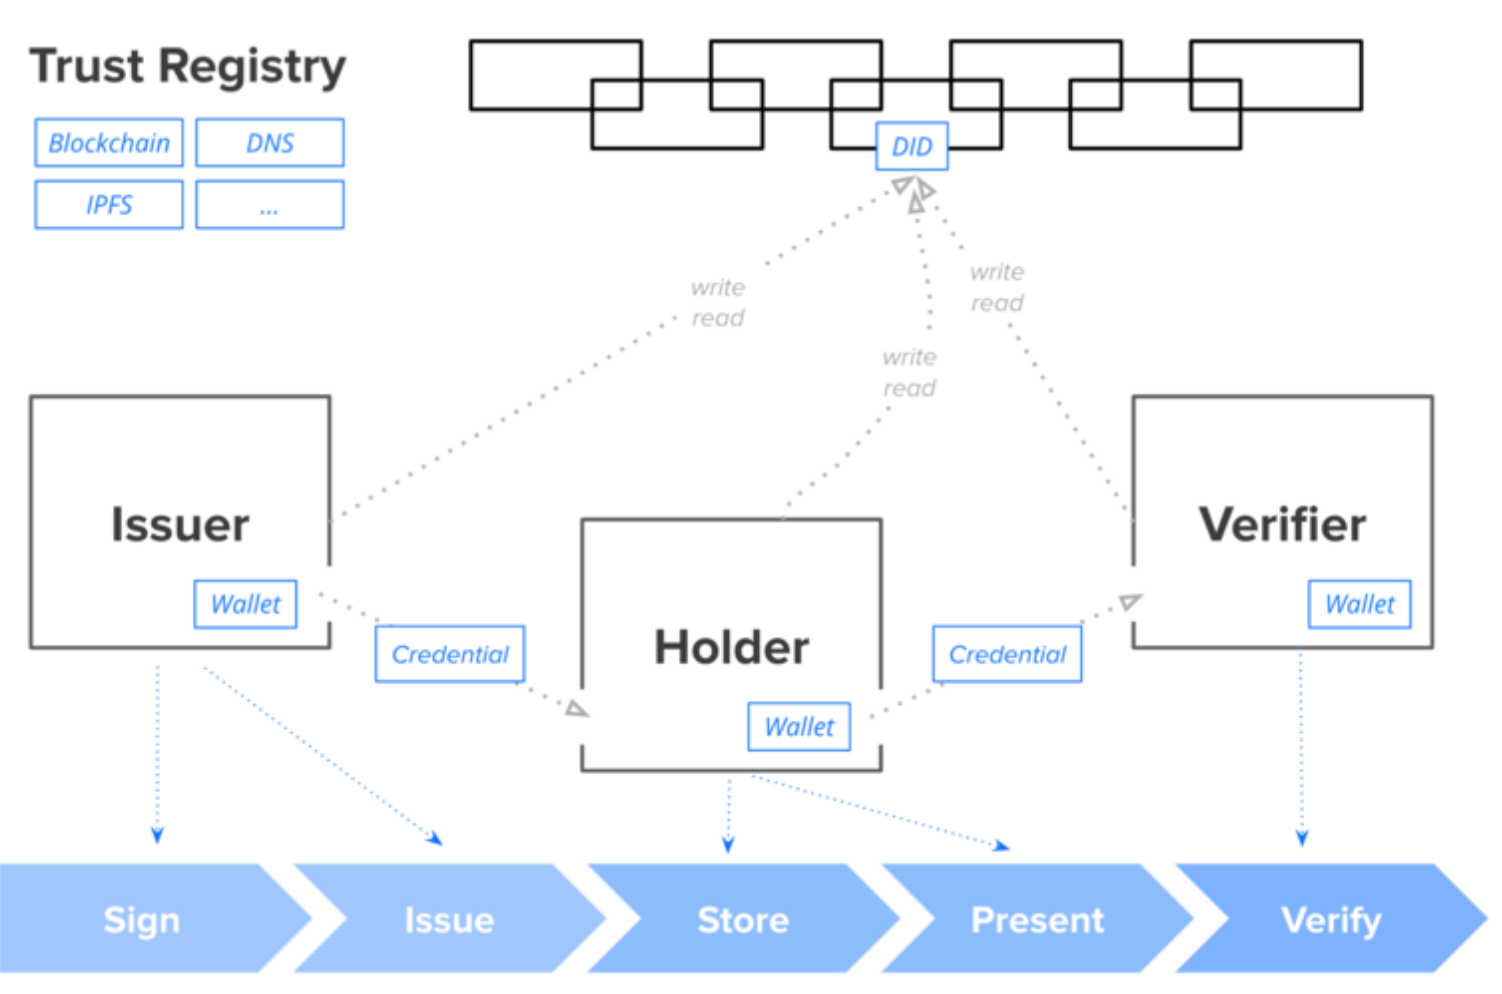
\includegraphics[scale=0.3]{media/zusammenspiel.png}
	\caption{Zusammenspiel von Issuer, Holder und Verifier}
	\label{fig:meine-grafik}
\end{figure}

Es ist zu erkennen, dass sowohl Issuer, Holder und Verifier Eigentümer von einem Wallet sind. Der Issuer (Beispielsweise eine Bank) stellt VC's aus, die der Holder (Beispielsweise eine Privatperson) in seinem Wallet speichert. Muss sich dieser nun ausweisen, so reicht er dem Verifier (Beispielsweise der Arbeitgeber) eine VC-Representation ein. Diese VC-Representation (oder auch Verifiable Presentation \textsl{VP} genannt) beinhaltet in der Regel ein VC, kann jedoch in komplexeren Szenarien mehrere VC's enthalten. Zudem ist der jeder (insbesondere der Verifier) in der Lage die Authentizität des VP zu überprüfen.\\

Issuer, Holder und Verifier können jeweils alle drei Rollen annehmen, besitzen eine DID und sind DID-Subjects. Folgende Zusammenhänge existieren zwischen dem DID-Subject, DID, DID-URL, DID-Controller, DID-Document und der Verifiable Data Registry:

\begin{figure}[h]
	\centering
	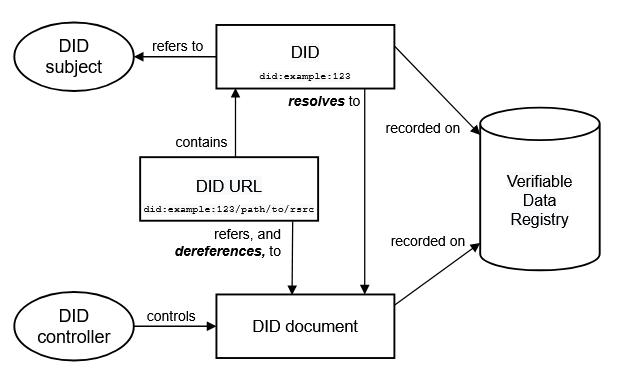
\includegraphics[scale=0.9]{media/DID.PNG}
	\caption{Zusammenspiel von Issuer, Holder und Verifier \cite{ID18}}
	\label{fig:meine-grafik}
\end{figure}

Die DID-URL beinhaltet die DID und erweitert die Syntax um die URI-Komponenten wie Pfade oder Anfrage-Parameter. Sowohl DID's als auch DID-Documents werden auf einem Verifiable Data Registry persistiert. Diese werden beispielsweise als Datenbanken oder dezentrale Dateisysteme realisiert. In diesem Kontext sind jedoch distributed Ledger die Speicher der Wahl. Das DID-Dokument wird durch die DID-URL (de-)referenziert und durch die DID auf sich verwiesen. Der DID-Controller ist die Entität, die das DID-Document modifizieren kann. In der Regel ist diese Entität das DID-Subject der DID, es kann jedoch auch ein ein oder mehrere andere DID-Subjecte sein.


\section{Politik, Recht und Ethik in Bezug auf SSI}

\subsection{Politik}
Aus politischer Sicht spielt SSI eine wichtige Rolle, da das Potential besteht das Monopol des Staates in Bezug auf die Ausstellung, Aufrechterhaltung und Entzug von Ausweisdokumenten zu verlieren. Durch die Einführung von digitalen Entitäten - mit denen man sich auch in der analogen Welt ausweisen könnte - können staatliche Institutionen nicht mehr uneingeschränkt über den genannten Prozess verfügen. Betroffen sein können unter anderem die Digitalisierung der Grenzkontrollen oder das Migrationsmanagement, indem Pässe, Visa und ähnliche Dokumente als VC zur Verfügung gestellt werden. \\
Eine weitere Auswirkung ist, dass durch SSI das aktuelle Monopol im Identitätsmanagement von Unternehmen wie Meta (Facebook) und Google durch föderierte Identitätsmanagementsysteme abgelöst wird. Dadurch haben letztere Unternehmen nicht mehr die Kontrolle über die Daten ihrer Nutzer, was auch monetäre Auswirkungen hat. Die zuvor für Marketingzwecke verwendeten Daten stehen demnach nicht mehr zu Verfügung für personalisierte Werbung und Ähnlichem.\\
Insgesamt hat SSI das Potenzial, das bestehende Identitätsmanagement-System zu revolutionieren und die Kontrolle über digitale Identitäten in die Hände der Nutzer zu legen. Dies wirkt sich auf verschiedene Bereiche aus, darunter die Politik, das Monopol des Staates, die Digitalisierung von Grenzkontrollen und die Monetarisierung von Daten.

\subsection{Recht}
Die Einführung von SSI wirft auch rechtliche Fragen und Aspekte auf. Eine zentrale Frage betrifft die rechtliche Anerkennung von digitalen Identitäten und die damit verbundenen Rechte und Pflichten. Da SSI die traditionelle Vorstellung von staatlich ausgestellten Ausweisdokumenten und Identitätsnachweisen herausfordert, müssen rechtliche Rahmenbedingungen geschaffen werden, um die Verwendung und den Schutz digitaler Identitäten zu regeln. Dies könnte die Festlegung von Standards für digitale Identitäten, Datenschutzbestimmungen, Haftungsfragen und den Zugriff auf und die Verwaltung von persönlichen Daten umfassen. Zudem muss auch geklärt werden, wie SSI in bestehende Rechtssysteme und -strukturen integriert werden kann, beispielsweise in Bezug auf Verträge, Gerichtsverfahren oder behördliche Angelegenheiten. Die rechtlichen Aspekte von SSI sind daher von großer Bedeutung, um die rechtliche Sicherheit, den Schutz der Privatsphäre und die Gewährleistung der Rechte und Pflichten aller beteiligten Parteien zu gewährleisten.\\
Weitere zu beachtende Aspekte sind die juristische Verantwortlichkeit oder Datenschutz. Vor allem Ersteres spielt eine Rolle, wenn es sich um die Verwendung von Identitätsinformationen, Identitätsdiebstahl oder Fälschungsversuchen handelt. Zweiteres ist relevant in Bezug auf die rechtlichen Anforderungen die mit Datenverwaltung einhergehen.

\subsection{Ethik}
Auch auf ethnischer Sicht zeigt sich die Relevanz von SSI. Gerade das Konzept der Dezentralisierung und die Tatsache, dass keine Instanz mehr Macht über die Identitäten hat als andere wirft ethnische Fragestellungen auf. In \cite{ID17} beschreibt Ishmaev das Paradoxon, dass einerseits SSI zuletzt genannte Eigenschaften fordert, jedoch andererseits verschiedene Levels an 'Vertrauen' an Entitäten in der analogen Welt existieren. So sind beispielsweise Dokumente, die von einer staatlichen Autorität zugewiesen werden bedeutender als das Sportabzeichen für Grundschüler. Dieser Zustand wird in dem SSI-Konzept jedoch nicht berücksichtigt und zeigt den Kompromiss, den SSI-Identitätsmanagementsysteme implementieren müssen.\\
Ein weiterer problematischer Aspekt, ist die von Ishmaev genannte Tatsache, dass die Macht über die Freigabe der Daten zwar bei dem Nutzer liegt, die Macht über die Nutzung eines Dienstes liegt jedoch weiterhin bei dem Anbieter. So kann ein Großkonzern für die Nutzung eines Dienstes eine unmoralische Menge an Informationen fordern. Dadurch wird klar, dass weiterhin eine problematische Machtrelation existiert.\\

Ein weiterer Punkt ist die Diskrepanz zwischen SSI im sozialen und im technischen Kontext. SSI-Systeme unterscheiden nicht zwischen den handelnden Entitäten, ob es sich um Privatpersonen, Institutionen oder - im Rahmen von Internet-of-Things - Hardware handelt. Gerade dadurch weißt die Interpretation von 'Vertrauen' in sozialen oder cybersecurity Bereich Unterschiede auf. Es gibt eine Vielzahl an Definitionen für "Vertrauen", wobei diese meist in Abhängigkeit zu dem Kontext stehen, in dem sie verwendet werden. Eine allgemeine Definition wurde von McKnight und Chervany (1996) festgelegt: Vertrauen ist der Grad zu welchem eine Partei einwilligt abhängig zu etwas oder jemanden in einer Situation zu sein mit einem Gefühl von Sicherheit. Hierbei werden explizit und implizit folgende drei Bestandteile von Vertrauen dargestellt \cite{ID24}:
\begin{itemize}
	\item Abhängigkeiten zwischen Parteien
	\item Zuverlässigkeit einer Partei
	\item Risiko, dass eine Partei nicht wie erwartet agiert
\end{itemize}
Alle diese drei Charakteristika unterscheiden sich, je nachdem ob es sich um IoT-Geräte, Software oder Menschen handelt. 


%----------------- KAPITEL : Distributed ledger Technology  ----------------- %
%\chapter{Distributed Ledger Technology}
\label{cha:distributedLedgerTechnology}

\section{Merkmale und Vorteile von DLT}
Distributed Ledger ist - wie der Titel bereits beschreibt - eine , für diese Arbeit, bedeutende Technologie. Dabei sind folgende Merkmale und Vorteile der DTL relevant \cite{ID19}:
\begin{itemize}
	\item DLT ermöglicht das Betreiben einer hochverfügbaren Datenbank (eines 'Ledgers'), da nicht eine zentrale Instanz für die Verfügbarkeit verantwortlich ist, sondern die Gesamtheit der Knoten in dem Netzwerk.
	
	\item Ebenso ermöglicht die Dezentralität des DLT eine verteilte Speicherung und Verarbeitung.
	
	\item Manipulationsresistenz wird durch kryptographische Verfahren innerhalb der Blockchain sichergestellt. Im Fall  der Blockchain sind sind sind diese in der Regel asymmetrische Verfahren, was bedeutet, dass private/öffentliche Schlüssel zum Ent- oder Verschlüsseln der Daten verwendet werden, wobei 'Integer Factorization', "Discrete Logarithm' oder 'Elliptic Curves' verwendet werden können \cite{ID23}
	
	\item Zensurresistenz kann gewährleistet, indem beispielsweise alle Knoten die gleichen Berechtigungen haben und somit keine machthabende Instanz existiert. Alle Teilnehmer im Netzwerk werden als Knoten (Nodes) bezeichnet und besitzen jeweils eine lokale Kopie des Ledgers. Änderungen werden nun auf der Kopie ausgeführt und im Anschluss in dem Netzwerk synchronisiert. Das Netzwerk gilt als "untrustworthy" (nicht vertrauenswürdig), wenn willkürliche einzelne Knoten sog. 'Byzantine-Failures' \cite{ID20} \cite{ID21} erzeugen können. Dies bedeutet, dass versucht wird beliebig falsches Verhalten im System zu erzeugen (unauthentische Daten, Zusammensturz des Systems, etc). Der Resistenzgrad des Netzwerks gegenüber diesen Angriffen wird als 'Byzantine-Toleranz' bezeichnet und wird in der Regel durch Abstimmungen im Netzwerk (Beispielsweise Konsensus-Algorithmen) verhindert. Beispiele im Blockchain-Kontext sind 'Proof-of-Work' oder "Proof-of-Stake' \cite{ID22} Algorithmen.
	
	\item Möglichkeit zur 'Demokratisierung' von Daten: Durch DLT kann ermöglicht werden, dass Individuen und/oder Organisationen kooperativ Kontrolle über Daten ausüben
	
\end{itemize}

\section{Anwendung von DLT im Bereich der digitalen Identität}
Die oben genannten Eigenschaften sind für das Betreiben eines Identitätsmanagementsystems optimal, da diese hochverfügbar sein sollten, mit möglichst kurzen oder nicht existierenden Downtimes. Auch ist eine verteilte Speicherung und Verarbeitung eine effiziente Möglichkeit große Menge an Anfragen zu bearbeiten oder eine Vielzahl an Identitätsdaten zu speichern. Zusätzlich ist Manipulationsresistenz von großer Bedeutung, da die Identitätsdaten stets authentisch sein müssen, um beispielsweise Dokumentenfälschung oder Identitätsdiebstahl zu vermeiden. Ebenso können finanzielle Transaktionen hiermit abgewickelt werden, was in der analogen Welt oft im Zusammenhang mit der Dokumentenausstellung stattfinden. Ein Beispiel hierfür sind die Gebühren beim Beantragen eines Reisepasses oder die Strafgebühr für das zu späte Neubeantragen eines Abgelaufenen Ausweises.
Die Möglichkeit sog. 'smart contracts' - also eigene Programme - zu schreiben ist eine Eigenschaft, die nicht in allen DLT's gegeben ist. Dennoch wird diese Eigenschaft an dieser Stelle erwähnt, da einige Blockchains wie Ethereum Letzteres unterstützen und somit einem Software-Entwickler die Chance geben fehlende Software im Identitätsmanagementsystems zu implementieren.

Diese Merkmale von DLT machen es zu einer idealen Technologie für die Umsetzung von Self-Sovereign-Identity. Sie ermöglicht eine sichere, vertrauenswürdige und selbstbestimmte Verwaltung von Identitätsinformationen, wodurch Benutzer die Kontrolle über ihre Identität zurückerlangen und die Notwendigkeit von zentralen, vertrauenswürdigen Dritten verringert wird.


%----------------- KAPITEL : Anforderungsanalyse  ----------------- %
\chapter{Anforderungsanalyse}

\section{Use-Case}
Der zu implementierende Use-Case ist, dass eine Autorität in der Lage sein muss einen Führerschein an einen Nutzer auszustellen. Der Führerschein darf für Niemand anderen als den Nutzer einsehbar sein. Es muss jedoch die Möglichkeit geben, dass eine andere Autorität den Führer auf Authentizität überprüft oder herausfinden kann, ob der Führerschein für die richtige Fahrzeugart ist oder wann der Fahrer den Führerschein erhalten hat. Von Bedeutung ist, dass nicht der ganze Führerschein gezeigt werden muss, sondern dass selektiv entweder einzelne Attribute einsehbar gemacht werden oder Anfragen bejaht/verneint werden. Sollte der Fahrer Fehlverhalten zeigen, so kann die Autorität den Führerschein wieder entziehen.

\label{cha:anforderungsanalyse}
Folgende Anforderungen gelten für das Identitätsmanagementsystem und entsprechen den von der OECD festgelegten Eigenschaften \cite{ID25} \cite{ID26}.
\section{Funktionale Anforderungen}
\begin{itemize}
	\item Widerruf: Nachdem ein Credential ausgestellt wurde muss die Möglichkeit existieren diesen zu widerrufen. Dies kann durch den Holder oder Issuer des Credentials geschehen. Dazu gehört auch, dass Credentials nach einer bestimmten automatisch ungültig sein können. Diese Fälle tretten ein, wenn beispielsweise der Nutzer ein hohes Alter erreicht und eigenständig freiwillig den Führerschein abgibt oder wenn die Gültigkkeit abläuft, weil der Nutzer zu alt ist. Auch muss der Führerschein entziehbar sein, wenn der Fahrer Fehlverhalten gezeigt hat (betrunken fahren, zu schnell, etc.).
	\item Überprüfbarkeit: Es muss möglich sein, dass ein Verifier Credentials überprüfen kann. Auch muss nachverfolgbar sein wann der Credential durch wen erstellt wurde. Wenn beispielsweise ein Führerschein als Credential ausgestellt wurde, so muss ein Kontrolleur in der Lage zu sein diesen auf Gültigkeit und korrekte Attribute zu prüfen.
	\item Selektive-Veröffentlichung: Dem Nutzer muss es möglich sein lediglich einzelne Claims zu veröffentlichen. In der analogen Welt zeigt der Kunde beispielsweise den kompletten Ausweis, obgleich nur das Alter überprüft werden möchte. Demnach soll die Funktion existieren ausschließlich eine Submenge von Informationen eines Credentials offen zu legen.
\end{itemize}

\section{Nicht-Funktionale Anforderungen}

\begin{itemize}
	\item Vertraulichkeit: Credentials müssen vor unbefugten Zugriffen geschützt sein. Gemeint ist hiermit, dass unberechtigte Nutzer Credentials weder schreiben noch lesen sollten.
	\item Integrität: Credentials dürften nur autorisiert modifiziert werden. Dies betrifft Claims eines Credentials oder den gesammten Credential.
	\item Non-Replay: Operationen dürfen nicht erneut ausführbar sein. Dies bedeutet, dass beispielsweise die Credential-Zuweisung nicht mehrfach ausgeführt werden kann, da ansonsten ein Holder entweder doppelte Credentials erhält oder ein zweiter (und somit unberechtigter) Holder ebenso den Credential fälschlicherweise empfangen kann.
	\item Nichtabstreitbarkeit: Die Transaktionen müssen dokumentiert sein, sodass Aktivitäten nicht abgesprochen werden können. Beispielsweise sollte der Issuer nicht in der Lage sein abzustreiten, dass ein Credential erstellt wurde.
	
\end{itemize}

\section{Technische Anforderungen}
Als technische Anforderung wird lediglich festgelegt, dass eine DLT verwendet werden soll, was in dieser Arbeit durch die Blockchain realisiert wird.
Bei den Templates für die Credentials, die beschrieben welche Attribute ein Dokument hat (z.B. Fahrzeugtyp im Führerschein) muss sich an den \textsl{W3C Standard für Verifiable Credentials} \footnote{https://www.w3.org/TR/vc-data-model/} gehalten werden. 

\include{chapter/darstellungExistierenderLösungen}

%\chapter{Vergleich existierender Lösungen}
\label{cha:vergleich Lösungen}
\section{Allgemein}
In der Folgenden Tabelle werden die Lösungen von \textbf{Luniverse}, \textbf{Dock}, \textbf{Polygon} und \textbf{Sovrin} miteinander verglichen. Betrachtet wird dabei die Blockchain und dessen Konsensus-Algorithmus, ob ein Knoten ohne zusätzliche Erlaubnis ein Validator werden kann, ob ZK-Proofs verfügbar sind und wo die Credentials gespeichert werden. Im Anschluss werden die Transaktionskosten betrachtet und die maximale Transaktionsfrequenz.

\begin{landscape}
	\begin{table}[h]
		\centering
		\begin{tabular}{cccccc}
			\toprule
			\textbf{Bezeichung} & {Blockchain} & {Konsensus-Algorithmus} & {Permissionless?}& {ZK-Proofs?} & {Speicherung}\\
			\midrule
			\rowcolor{lavender}
			Luniverse 	& Luniverse-Sidechain 	& LPOA														& No 									& Yes 															& Wallet\footnote{Wird mit WalletSDK implementiert}					\\
			Dock      	& Dock-Sidechain		& GRANDPA													& No 									& Yes 															& Wallet\footnote{Wird mit WalletSDK implementiert}					\\
			\rowcolor{lavender}
			PolygonId 	& Polygon PoS 			& Proof-of-Stake 											& Yes 									& Yes 															& PolyginId App oder WalletSDK										\\
			Sovrin 		& Sovrin Network 		& Plenum\footnote{Basiert auf 'Byantine Failt Tolerance'} 	& No 									& Yes 															& WalletSDK															\\
			\rowcolor{lavender}
			ShoCard 	& Bitcoin				& Proof-of-Work 											& Yes 									& No 															& Blockchain, ShoCard central server, App							\\
			\bottomrule
		\end{tabular}
	\end{table}
\end{landscape}


\section{Transaktionskosten}
Transaktionen auf der Blockchain sind Prozesse, die in den verteilten Speicher schreiben. Da Transaktionen von Validator-Knoten überprüft werden, muss an das Netzwerk eine Gebühr gezahlt werden. Diese variiert je nach Blockchain, Zustand der Blockchain und Auslastung.
\begin{itemize}
	\item Luniverse: Luniverse gibt an, dass keine Transaktionsgebühren existieren.
	\item Dock: Gibt an, dass keine Gebühren anfallen für die Credentialerstellung. Transaktionen für das erstellen von Schemas oder Credentials widerrufen seien sehr gering \cite{ID44}
	\item Polygon: Bei Polygon lassen sich die Transaktionskosten sehr genau berechnen. Dabei hängt es von zwei Faktoren ab, wie teuer die Transaktion wird \cite{ID45}:
	\begin{itemize}
		\item Menge an Gas: Das ist eine Metrik für die Leistung, die das Netzwerk für das Ausführen der Transaktion zur Verfügung stellt. Im Falle vom Polygon wird die 'Ethereum Virtual Machine' (EVM) verwendet, welche Platten-Verwendung, CPU-Verwendung, etc. misst und so die Menge an Gas berechnet.
		\item Gaspreis: Dieser Faktor hängt von der Netzwerkauslastung ab. Prinzipiell gibt es drei Modelle zwischen denen man entscheiden muss: Standard, Fast und Rapid. Dabei wird aufsteigend die Transaktionsdauer geringer (30-10 bei Standard und 5-10 bei Rapid). Analog dazu steigt auch der Gaspreis. Auf PolygonScan\footnote{https://polygonscan.com/gastracker} können die Gaspreise historisch betrachtet werden.
	\end{itemize}
	\item Sovrin: Credential und DID-Erstellung sind kostenlos. Für alles andere (also Revokation, Schemas, etc) gibt es jeweils für TestNet und MainNet eigene Preise.
	\item ShoCard: Transaktionskosten auf der Bitcoin Blockchain werden in Satoshi ($1 * 10^{-6} Bitcoin$) pro Byte berechnet. Demnach kostet die Transaktion mehr, je nachdem viele Daten in die Blockchain geschrieben werden. Im Jahr 2023 betrugen die Kosten für eine Transaktion im Durchschnitt zwischen einen und drei Euro \cite{ID49}. Es ist jedoch anzunehmen, dass Transaktionen, die Data-Anchoring betreiben, mehr kosten, da mehr Daten geschrieben werden.
	
\end{itemize}

\section{Konsensus-Algorithmus}
Konsensus-Algorithmen werden verwendet, um einen einheitlichen Zustand des Netzwerk zwischen den Knoten festzulegen. Hierbei gibt es verschiedene Ausführungen, die im Folgenden betrachtet werden:
\begin{itemize}
	\item LPOA: Dieses Akronym steht für "Luniverse's Proof of Authority" \cite{ID50}. Hierbei handelt es sich um einen Proof-of-Authority-Algorithmus, wo ein Validator nicht anhand seiner zur Verfügung gestellten Rechenkraft oder Kryptowährung bemessen wird, sondern an seiner Identität. Potentielle Validatoren (beispielsweise Unternehmen, Institutionen, Regierungen, etc.) müssen sich bei einer Einrichtung oder Organisation, die das PoA-Netzwerk betreibt, bewerben oder eingeladen werden. Diese entscheiden anhand der Reputation und der Vertrauenswürdigkeit des Bewerbers, ob dieser als Validator fungieren darf. Sollte Letzteres erlaubt werden, so werden Verträge verfasst, um die Verantwortlichkeiten im Netzwerk festzulegen. Im Anschluss kann mit dem Validieren von Blöcken begonnen werden. Sollte Fehlverhalten des Validators festgestellt werden, so kann dieser aus dem Netzwerk ausgeschlossen werden \cite{ID51}.
	\item GRANDPA: Dieser Algorithmus lässt sich ebenso als Proof-of-Authority-Algorithmus klassifizieren
	\item Proof-of-Stake: Proof of Stake (PoS) ist ein Konsensusmechanismus in Blockchain-Netzwerken, der verwendet wird, um Transaktionen zu validieren und neue Blöcke zur Blockchain hinzuzufügen. Im Gegensatz zu Proof of Work (PoW), bei dem Miner rechenintensive Aufgaben lösen müssen, um Blöcke zu erstellen, basiert PoS auf dem Konzept des "Stakings" oder des Einsatzes von Kryptowährungen.
	\begin{enumerate}
		\item \textbf{Validatoren und Staking:} In einem PoS-Netzwerk gibt es keine Miner im herkömmlichen Sinne. Stattdessen gibt es Validatoren. Um ein Validator zu werden, müssen Benutzer eine bestimmte Menge der Kryptowährung des Netzwerks als Einsatz hinterlegen. Dieser dient als Garantie dafür, dass der Validator korrekt arbeitet.
		
		\item \textbf{Blockvalidierung:} Wenn eine Transaktion im Netzwerk eingereicht wird, wird ein Validator zufällig ausgewählt, um die Transaktion zu validieren und einen neuen Block hinzuzufügen. Die Wahrscheinlichkeit, ausgewählt zu werden, hängt oft von der Menge des gestakten Vermögens ab, was bedeutet, dass Benutzer mit größeren Stakes eine höhere Chance haben, ausgewählt zu werden.
		
		\item \textbf{Belohnungen:} Validator, die korrekt arbeiten und Transaktionen ordnungsgemäß validieren, erhalten Belohnungen in Form von Transaktionsgebühren und neuen Kryptowährungseinheiten, die dem System hinzugefügt werden. Diese Belohnungen werden oft proportional zur Höhe des gestakten Vermögens des Validators verteilt.
		
		\item \textbf{Bestrafungen:} Wenn ein Validator betrügerisches Verhalten zeigt oder versucht, das Netzwerk zu schädigen, kann er seine gestakten Vermögenswerte verlieren oder andere Strafen erhalten.
	\end{enumerate}
	PoS \cite{ID53}bietet mehrere Vorteile, darunter eine geringere Umweltauswirkung im Vergleich zu PoW, da keine rechenintensiven Aufgaben erforderlich sind, und eine höhere Skalierbarkeit. Trotz der vielen Vorteile von Proof-of-Stake gibt es auch einige Nachteile \cite{ID53}:
	
	\begin{enumerate}
		\item \textbf{Zentralisierungstendenzen:} PoS kann zu einer gewissen Zentralisierung führen, da Teilnehmer mit großen Stakes mehr Einfluss haben und wahrscheinlicher ausgewählt werden, um Transaktionen zu validieren und Blöcke hinzuzufügen. Dies könnte zu einer Konzentration der Netzwerkvalidierungsmacht führen.
		
		\item \textbf{Reichtumsungleichheit:} PoS belohnt Benutzer proportional zu ihren gestakten Vermögenswerten. Dies könnte die bestehende Reichtumsungleichheit in Kryptowährungen weiter verstärken, da reichere Benutzer größere Stakes halten können und somit mehr Belohnungen erhalten.
		
		\item \textbf{Gefahr von Auslagerung (Staking as a Service):} Einige Benutzer könnten ihre Staking-Aktivitäten an Dritte auslagern, um die Belohnungen zu maximieren. Dies könnte dazu führen, dass reiche Benutzer Dritte beauftragen, um ihre Stakes zu verwalten, was die Dezentralisierung gefährden könnte.
		
		\item \textbf{Geringe Anreize für Aktivität:} Einige PoS-Netzwerke könnten Schwierigkeiten haben, Benutzer dazu zu ermutigen, aktiv am Netzwerk teilzunehmen, da sie bereits gestakte Vermögenswerte besitzen und möglicherweise keine zusätzlichen Anreize sehen, aktiv Transaktionen zu validieren.
		
		\item \textbf{Schwierigkeiten bei der Wahl der Validatoren:} Die Auswahl von zuverlässigen und ehrlichen Validatoren kann eine Herausforderung darstellen. Es müssen Mechanismen implementiert werden, um sicherzustellen, dass betrügerische oder bösartige Validatoren erkannt und bestraft werden.
		
		\item \textbf{Sicherheitsprobleme bei geringer Beteiligung:} PoS-Netzwerke könnten anfällig für Angriffe sein, wenn die Beteiligung gering ist und nur wenige Validatoren vorhanden sind. In solchen Fällen könnten Angreifer leichter die Kontrolle über das Netzwerk erlangen.
		
		\item \textbf{Verlust von gestakten Vermögenswerten:} Bei fehlerhaftem Verhalten oder betrügerischen Handlungen können Validatorn Strafen auferlegt werden, einschließlich des Verlusts ihrer gestakten Vermögenswerte.
	\end{enumerate}
	
	\item Proof of Work (PoW) ist ein Konsensusmechanismus, der in vielen Blockchain-Netzwerken verwendet wird. Er dient dazu, Transaktionen zu validieren, neue Blöcke zur Blockchain hinzuzufügen und das Netzwerk vor verschiedenen Arten von Angriffen zu schützen. Im Folgenden sind die Grundlagen von PoW zu betrachten:
	
	\begin{enumerate}[label=\arabic*.]
		\item \textbf{Transaktionen validieren:} Im Netzwerk werden Transaktionen von Benutzern gesammelt und in einen Pool gestellt, der darauf wartet, in einen neuen Block aufgenommen zu werden. Diese Transaktionen müssen validiert werden, um sicherzustellen, dass sie den Regeln des Netzwerks entsprechen.
		
		\item \textbf{Rätsellösung:} PoW erfordert von den sogenannten Minern, mathematische Rätsel zu lösen, die als "Proof of Work" bezeichnet werden. Diese Rätsel sind so konzipiert, dass sie eine erhebliche Rechenleistung erfordern und gleichzeitig leicht zu überprüfen sind, sobald sie gelöst sind. Minen ist also ein wettbewerbsfähiger Prozess, bei dem die Miner darum konkurrieren, das Rätsel zu lösen.
		
		\item \textbf{Wettbewerb und Belohnungen:} Die Miner verwenden ihre Rechenleistung, um das Rätsel zu lösen. Der erste Miner, der das Rätsel erfolgreich löst, kann einen neuen Block erstellen und ihn mit den validierten Transaktionen füllen. Dieser neue Block wird dann der Blockchain hinzugefügt. Als Belohnung für ihre Arbeit erhalten die Miner neue Kryptowährungseinheiten (z. B. Bitcoin) sowie die Transaktionsgebühren, die von den Benutzern für die Validierung ihrer Transaktionen gezahlt werden.
		
		\item \textbf{Sicherheit und Dezentralisierung:} PoW schützt das Netzwerk, indem es für Angreifer sehr teuer macht, die Mehrheit der Rechenleistung im Netzwerk zu kontrollieren. Je mehr Rechenleistung ein Angreifer benötigt, desto schwieriger wird es, das Netzwerk zu übernehmen. Dies trägt zur Sicherheit und Dezentralisierung bei, da viele Miner weltweit am PoW-Prozess teilnehmen.
		
		\item \textbf{Schwierigkeitsanpassung:} Das PoW-System passt die Schwierigkeit des zu lösenden Rätsels automatisch an die Gesamtrechenleistung des Netzwerks an. Dies stellt sicher, dass die Zeit zwischen der Erstellung neuer Blöcke ungefähr gleich bleibt, unabhängig davon, wie viele Miner im Netzwerk aktiv sind.
	\end{enumerate}
	
	Obgleich PoW mit vielen Vorteilen einhergeht stehen auch Kritikpunkte im Raum: Unter anderem ist PoW höchst ineffizient, da wie bereits erwähnt nur der erste Miner, der das Rätsel löst belohnt wird, obwohl viele andere Miner gleichzeitig am selben Problem arbeiteten. Dadurch werden große Mengen an Rechenleistung verschwendet. 
	
	
	
\end{itemize}

%----------------- KAPITEL : System-Design  ----------------- %
\chapter{System-Design}
\label{cha:systemdesign}

\section{Architektur des dezentralen Identitätsmanagementsystems Anforderungen}
\blindtext

\section{Komponenten und deren Funktionalitäten}
\blindtext

\section{Interaktion zwischen den Komponenten}
\blindtext

\section{Integration von DLT in das Systemdesign}
\blindtext


%----------------- KAPITEL : Implementierung  --------------------- %	
%\chapter{Implementierung}
\label{cha:implementierung}

\section{Auswahl geeigneter DLT}
\blindtext

\section{Ausführung von Performance-Tests}
\blindtext

\section{Implementierung}
\blindtext

\section{Sicherheitsmechanismen}
\blindtext


%----------------- KAPITEL : Evaluation  --------------------- %	
\chapter{Evaluation}
\label{cha:evaluation}

\section{Festlegen der Evaluations Metriken}
Folgende Metriken werden im folgenden Betrachtet:
\begin{itemize}
	\item Laufzeit
	\item Sicherheit
\end{itemize}
\subsection{Metrik - Laufzeit}
Um die Laufzeit der Operationen zu messen wurde ein Python-Script entwickelt, welches die Operationen 'createIdentity', 'getIdentity', 'createClaim' und 'getClaimQR' jeweils 100 mal ausführt. Jeder Aufruf startet einen eigenen Subprozess mit dem Python Framework 'subprocess', welcher mit dem Framework 'timeit' gemessen wird. Gemessen wird der Durchschnitt und der Median bei jeweils 100 Ausführungen einer Operation. Die gemessenen Werte sehen wie folgt aus:

\begin{center}
	\begin{tabular}{ c c c }
		Operation\_Name & Durchschnitt & Median \\
		createClaim & 1.2098522 & 1.0454559 \\
		createIdentity & 1.1128388 & 1.1019622  \\
		getClaimQR & 1.5566253 & 1.2646243 \\
		getIdentity & 1.1031939 & 1.0355741 \\
	\end{tabular}
\end{center}
Es ist zu erkennen, dass der Median in jedem Fall geringer ausfällt als der Durchschnitt. Dies muss damit zusammenhängen, dass ein Teil der Aufrufe unverhältnismäßig länger dauern.\\

Der folgenede Code zeigt wie die Messung der Laufzeit stattgefunden haben.

\begin{lstlisting}[language=python]
	def runMeasurement(command, cache):
		runs = 100
		key = command.split()[3]  # "node app -a createIdentity" -> createIdentity
		try:
			runtime = timeit(stmt="subprocess.call('{}')".format(command), setup="import subprocess", number=runs, )
			durations = repeat(stmt="subprocess.call('{}')".format(command), setup="import subprocess", number=1, repeat=runs)
		
			cache[key + "_median"] = calcMedian(durations)
			runtime = checkisFloat(runtime)
			if runtime:
				cache[key + "_average"] = runtime
		except:
			pass  # the error here can be ignored
			
	cache = {}
	runMeasurement(create_identity_command, cache)
	runMeasurement(get_identities_command, cache)
	runMeasurement(create_claim_command.format("Truck", "2000", first_identifier), cache)
	runMeasurement(get_claim_command.format(first_claim, first_identifier), cache)	
\end{lstlisting}	

\section{Sicherheitsevaluierung}
Die Komponente, die den größten Schutz in der Implementierung benötigt ist der Issuer. Das SSI-Konzept ist abhängig davon, wie vertrauenswürdig der Issuer ist. Daher findet eine Security-Analyse nach dem STRIDE-Modell \cite{ID59}.

\subsection{Spoofing}
\label{Spoofing}
Dieser Angriff beschreibt unberechtigten Zugriff auf die Komponente. Hiergegen wurde implementiert, dass der Zugriff (der über ngrok stattfindet) nur authentifiziert passieren kann: --basic-auth 'ngrok:issecure' --basic-auth='username:password'. Zusätzlich besitzt die verwendete REST-API eine Basic-Authentifikation. Daher ist diese Komponente doppelt geschützt. Es wird stark empfohlen, dass die Passwörter den Richtlinien des BSI entsprechen \cite{ID60}.

\subsection{Tampering}
Dieser Angriff beschreibt die ungewollte Manipulation von Daten. Prinzipiell gibt können zwei Komponenten Daten verändern:
\begin{enumerate}
	\item Der Holder: Als Besitzer der Daten hat der Holder die Möglichkeit seine Credentials zu löschen. Dieser Prozess würde über die Applikation passieren, welche zunächst über ein potentielles Password des Geräts und zum anderen durch das Passwort der PolygonId-App geschützt ist.
	\item Der Issuer: Der Issuer kann ebenso Credentials revoken (widderufen). Aber wie bereits im Kapitel \ref{Spoofing} beschrieben ist der Issuer geschützt.
	\item Der Verifier: Hat keine Möglichkeit Credentials zu modifizieren und ist daher nicht weiter zu betrachten
\end{enumerate}

\subsection{Repudiation}
\label{Repudiation}
Dieser Angriff beschreibt, dass ein Nutzer eine Aktivität abstreiten kann. Gegen diese Attacke schützt die Blockchain, die jede Transaktion in der Blockchain speichert. Durch das Monitoring-Tool von Alchemy oder im Blockchain-Browser können diese Transaktionen betrachtet werden. Eine solche Transaktion kann wie folgt aussehen:

\begin{lstlisting}[language=json,firstnumber=1]
{
	"jsonrpc": "2.0",
	"id": 0,
	"method": "eth_call",
	"params": [
	{
		"from": "0x0000000000000000000000000000000000000000",
		"to": "0x134b1be34911e39a8397ec6289782989729807a4",
		"data": "0x7c1a66de0a79f724bb72300544255781fc350952acb21cb77ea9a719c8eebb7d1a055ad0"
	},
	"latest"
	]
}
\end{lstlisting}	
Es ist zu sehen, dass sowohl übertragene Daten, als auch involvierte Adressen gespeichert werden. Das Schreiben ist ebenso kryptographisch geschützt.

\subsection{Information disclosure}
\label{disclosure}
Dieser Angriff beschreibt das ungewollte Veröffentlichen von Daten. In diesem Prototypen gibt es vier Typen von Daten:
\begin{enumerate}
	\item Daten im Issuer: Diese Daten sind streng geheim und werden unter anderem in '.env' Dateien oder in einem Vault gespeichert. Darunter sind private Schlüssel, API-Schlüssel für Alchemy, Nutzernamen und Passwörter für UI und API. Zusätzlich liegen alle diese Daten in einer virtuellen Maschine, die mit 2-Faktor-Authentifizierung und einem 20-Stellen Root-Passwort geschützt sind.
	\item Daten in der Blockchain: Diese Daten sind bereits öffentlich.
	\item Daten im Holder: Die Daten werden in der Wallet-App gespeichert. Darunter sind private Schlüssel und die Credentials, welche durch ein Passwort in der Polygon-App geschützt sind.
	\item Daten im Verifier: Der Verifier benötigt lediglich Zugang zu den Schemas, welche öffentlich gespeichert sind, und einen RPC-Node, welcher in Umgebungsvariablen lokal gespeichert ist.
\end{enumerate}
Daher lässt sich erkennen, dass private Daten sicher gespeichert sind und nicht veröffentlicht werde können.

\subsection{Denial of service}
Denial of Service beschreibt eine Attacke, in die komplette Software oder Teile davon ungewollt außer Betrieb genommen werden. Dieser Angriff findet in dem Prototypen nur Anwendung in dem Verifier, da andere Komponenten entweder lokal sind, oder nur der Nutzer Zugriff hat. Im Verifier könnte ein Angreifer probieren den RPC-Node zu überlasten. Jedoch hat Alchemy hiergegen Mechanismen entwickelt \cite{ID61}.

\subsection{Evelation of priviledge}
Dieses Konzept beschreibt, dass ein Nutzer ungewollt seine Rechte auf ein höheres Level setzten kann, um autorisiert zu sein neue Aktivitäten auszuführen. Diese Art der Attacke findet jedoch keine Anwendung, da es keine Levels an Rechten gibt.

\subsection{Zusammenfassung - STRIDE}
\begin{center}
	\begin{tabular}{ c c }
		KATEGORIE & Abgesichert? \\
		Spoofing & \checkmark \\
		Tampering (Manipulation) & \checkmark \\
		Repudiation (Nichtanerkennung) & \checkmark\\
		Information disclosure (Veröffentlichung von Informationen) &\checkmark\\
		Denial of service & \checkmark\\
		Evelation of priviledge (Erhöhung von Rechten) & \checkmark \\
	\end{tabular}
\end{center}
Es ist zu erkennen, dass der Prototyp sicher ist im Rahmen des STRIDE-Modells.

\section{Beantworten der Forschungsfragen}
Im Folgenden werden die in Kapitel \ref{forschungsfragen} gestellten Fragen beantwortet:
\begin{enumerate}
	\item Es ist möglich Daten privat und öffentlich zu speichern. Dies passiert zum einen bei Shocard in dem Prozess des Bootstrapping (siehe \ref{shocard}) und zum andere bei zk-Proofs in PolygonId. Jedoch ist es zu empfehlen, private Daten wie Credentials auch privat zu speichern, wie es bereits in verschiedenen Lösungen angewandt wird.
	\item Dies hängt von dem Typ der Daten ab (siehe \ref{disclosure}
	\item Der Nutzer ist nun in der Lage zum einen eigene Credentials auszustellen und zum anderen diese zu verifizieren.
	\item Ja das Problem der Fake-User kann hiermit gelöst werden. Beispielsweise kann bei der Registrierung die Verifizierung eines Credentials erfolgen, wobei dieser Credential nur von einer autorisierten Instanz ausgestellt werden kann.
	\item Sollte der Nutzer den privaten Schlüssel seines Identity-Wallets verlieren, so existiert eine Recovery-Option, bei welcher der User - die bei der Erstellung angezeigten Passwörter - erneut angeben muss. Sollte der Nutzer den privaten Schlüssel an einen Angreifer preisgeben, dann ist der Wallet unbrauchbar.
	\item Revokation kann der User selber oder der Issuer durchführen
	\item Dieser Faktor stellt sich nicht als Problem, sondern sogar als Feature heraus. Nutzer (auch Issuer) können mehrere DIDs besitzen. Bei Sovrin (siehe \ref{sovrin}) wird pro Interaktion eine neue DID verwendet, um maximale Privatsphäre zu gewährleisten.
	\begin{enumerate}
		\item Proof-of-Stake stellte sich als passender Algorithmus herraus (siehe \ref{PolygonPOS})
		\item PolygonId verwendet eine öffentliche Blockchain (siehe \ref{PolygonPOS})
		\item Private Schlüssel des Issuers befinden sich in einem Vault (siehe \ref{vault}) und private Schlüssel des Users befinden sich in der Applikation des Mobilgeräts.
		\item Es wird eine permissionless Blockchain verwendet (siehe \ref{PolygonPOS})
		\item Ja, die Credentialausstellung ist leicht erweiterbar mit der Zustellung eines NFTs. Dies könnte sowohl on-chain im smartcontract geschehen oder in der REST-API des Issuers. Beide Komponenten sich beliebig erweiterbar.
		\item zk-Proofs werden vom Holder erstellt und an den Verifier gesendet, welcher diese überprüfen kann
	\end{enumerate}
\end{enumerate}

\section{Erfüllung der Anforderungen}
Die in Kapitel \ref{cha:anforderungsanalyse} gestellten Anforderungen werden die folgt erfüllt:
\begin{enumerate}
	\item Widerruf: Wird durch den Holder und Issuer ermöglicht
	\item Überprüfbarkeit: Der Holder kann zk-Proofs ausstellen, die der Verifier überprüfen kann
	\item Selektive Veröffentlichung: Wird zum einen durch 'selective disclosure' und zum anderen durch speichern von Credentials im öffentlichen Profil ermöglicht.
	\item Vertraulich: Mittels Passwörter und kryptographischen Verfahren ist diese Anwendung vertraulich
	\item Non-Replay: Jede Transaktion/Operation erfolgt authentifiziert und ist daher nicht reproduzierbar
	\item Nichtabstreitbarkeit: Ist gegeben (siehe \ref{Repudiation})
	\item Diebstahlschutz: Ist gegeben (siehe \ref{Spoofing} und \ref{disclosure}
	\item W3C-Standard : Wird erfüllt (auch ersichtlich im Schema 'xsd: http://www.w3.org/2001/XMLSchema')
\end{enumerate}
Es wird also ersichtlich, dass alle Anforderungen erfüllt wurden.
\section{Analyse der Ergebnisse}
Als Ergebnis der Analyse lässt sich sagen, dass eine Anwendung implementiert wurde, die zum einen sicher ist gegen verschiedene Typen an Attacken ist und zum anderen Performant, wobei erwähnt werden muss, dass die Performance größtenteils abhängig ist von der Performance der Issuer-Node-API und der Transaktionsgeschwindigkeit der Blockchain. Davon abgesehen sind alle Security-Richtlinien, Funktionalen/Nicht-Funktionalen/Technischen Anforderungen erfüllt.




%----------------- KAPITEL : Diskussion  --------------------- %	
%\chapter{Diskussion}
\label{cha:diskussion}

\section{Zusammenfassen der Ergebnisse}
\blindtext

\section{Vergleich mit vorhandenen Ansätzen}
\blindtext

\section{Potenziale und Herausforderungen des dezentralen Identitätsmanagementsystem}
\blindtext

\section{Ausblick auf zukünftige Forschungsrichtungen}
\blindtext


%----------------- KAPITEL : Fazit  --------------------- %	
\chapter{Fazit}
\label{cha:fazit}

\section{Zusammenfassung der Arbeit}
Diese Thesis nimmt eine tiefgehende Betrachtung der Problematik vor, die mit herkömmlichen Identitätsmanagementsystemen in der heutigen vernetzten Welt einhergeht. Sie identifiziert und analysiert den wachsenden Bedarf für SSI und legt einen besonderen Fokus auf die technischen Grundlagen dieses Ansatzes.

Zu Beginn wurden die Grundlagen und die historische Entwicklung von Identitätsmanagementsystemen beleuchtet. Diese umfassen sowohl zentrale als auch dezentrale Ansätze, wobei letztere im Kontext von SSI von besonderem Interesse sind. Die Thesis beschäftigt sich ausführlich mit den technischen Grundlagen von SSI, einschließlich der Konzepte von Holder (Identitätsinhaber), Issuer (Identitätsaussteller) und Verifier (Identitätsüberprüfer). Dieser theoretische Rahmen bildet die Grundlage für das Verständnis und die Implementierung von SSI.

Ein zentraler Aspekt dieser Arbeit ist die Bedeutung von Distributed Ledger Technology (DLT) für die Umsetzung von SSI. Die Verwendung von DLT ermöglicht es, Identitätsdaten sicher und dezentral zu speichern, wodurch die Kontrolle über persönliche Informationen wieder in die Hände der Nutzer gelegt wird. Die Thesis untersucht verschiedene DLT-Plattformen und deren Eignung für die Implementierung von SSI, wobei die Wahl auf Polygon als Technologie fällt.

Das Design des SSI-Prototyps wird im Detail erläutert, wobei die Interaktion zwischen den verschiedenen Komponenten des Systems eine entscheidende Rolle spielt. Ein spezifisches Szenario wird ausgewählt und umgesetzt, um die praktische Anwendung von SSI aufzuzeigen.

Eine umfassende Evaluierung des Prototyps erfolgt anhand verschiedener Metriken, darunter die Laufzeit und Sicherheit. Neben den Metriken wird auch die Erfüllung der Anforderungen im Detail betrachtet.

\section{Erfüllung der Zielsetzung}
Die in Kapitel \ref{zielsetzung} gesetzte Zielsetzung  wurde vollständig erfüllt. Es wurde - wie beschrieben - ein dezentrales Identitätsmanagementsystem entwickelt, welches DLT implementiert. Hierbei ist - wie gefordert - der Nutzer Herrscher über seine Daten. Sowohl die funktionalen/nicht-funktionalen als auch technischen Anforderungen wurden erfüllt. Zudem sind Sicherheit, Kontrollierbarkeit und Skalierbarkeit berücksichtigt worden. Auch das vorgestellte Szenario kann ausgeführt werden - implementiert wurde es doch Anhand eines Führerschein-Beispiels.


\section{Diskussion}
In dieser Arbeit gab es mehrere Optionen das in der Zielsetzung beschriebene Ziel zu implementieren. Wäre die Anwendung beispielsweise nicht im Polygon Framework implementiert worden, so wäre Dock eine valide Alternative gewesen. Der Vorteil hierbei ist, dass keine eigenen Issuer-Knoten oder ähnliches gehostet werden müssen und viele Dienste bereits implementiert wurden, wie das Zuschicken von Credentials über Email - direkt an mehrere Empfänger. Auch ist ein Vorteil, dass die Dock-REST-API viele SSI-Methoden bereits anbietet, wie das Erstellen und Widerrufen von Credentials, Erstellen von Schemas, etc.\\
Auch wäre es in der implementierten Lösung bedenkenswert den Issuer oder Verifier nicht off-chain sondern on-chain zu implementieren. Hierbei befände sich die Logik im Smartcontract und gibt die Möglichkeit Operationen direkt in der Blockchain durchzuführen (Token-Transfer, Verwendung anderer Smart-Contracts, bessere Nachverfolgbarkeit, etc.). Auch wäre es denkbar einen eigenen Identity-Wallet zu implementieren und zu verwenden. In der hier vorgestellten Lösung wurde die PolygonId-App verwendet, jedoch stehen mehrere SDK zur Verfügung, womit ein Entwickler seinen eigenen Wallet erstellen kann.\\
Zusätzlich gibt es das Konzept der Non-Fungible-Token, die mit dem Proof-Of-Ownership-Gedanken dem SSI-Konzept ähneln. Daher wäre es abwägbar, ob eine Integration von NFT's in eine weiterführende Arbeit von Bedeutung wäre.


\section{Zukünftige Forschungsrichtungen}
Der Blick in die Zukunft des Forschungsfelds im Bereich SSI und deren Implementierung mithilfe von Distributed Ledger Technology (DLT) verspricht faszinierende Entwicklungen. In den kommenden Jahren werden Forscher voraussichtlich verstärkt die Skalierbarkeit von SSI-Systemen erforschen, um diese für breitere Anwendungsbereiche tauglich zu machen. Ein Schwerpunkt könnte dabei auf der Integration von SSI in bestehende digitale Infrastrukturen und Plattformen liegen, um die nahtlose Interoperabilität zu gewährleisten.

Des Weiteren wird die Verbesserung der Sicherheitsaspekte von SSI von entscheidender Bedeutung sein. Forschung wird sich auf fortschrittliche Kryptographie, Authentifizierungsmethoden und Datenschutzkonzepte konzentrieren, um das Vertrauen in diese Systeme zu stärken und Datenschutzverletzungen zu minimieren.

Die Entwicklung von internationalen Standards und Protokollen für SSI wird eine weitere wichtige Forschungsrichtung sein. Diese Standards sind entscheidend, um die weltweite Akzeptanz und Anwendung von SSI-Systemen zu fördern und Interoperabilität zwischen verschiedenen Implementierungen sicherzustellen.

Schließlich werden auch soziale und ethische Aspekte der Selbstsouveränen Identitäten verstärkt in den Fokus rücken. Forschung wird sich auf Fragen der Akzeptanz, der Bildung und Sensibilisierung der Nutzer, sowie auf die ethischen Implikationen in Bezug auf Identitätsmanagement und Datenschutz konzentrieren.

Insgesamt versprechen zukünftige Forschungsrichtungen auf dem Gebiet der Selbstsouveränen Identitäten und DLT eine spannende und vielversprechende Entwicklung, die sowohl technische als auch gesellschaftliche Herausforderungen angehen wird, um die Vision von selbstsouveränen und sicheren Identitäten in einer digitalisierten Welt voranzubringen.

\section{Beitrag zur Forschung}
Diese Arbeit leistet deutende Beiträge zur Forschung im Bereich 'Dezentrale Identitätsmanagementsysteme', da zunächst mehrere existierende Lösungen vorgestellt und verglichen wurden. Dabei wurden unterschiedliche Konzepte zur Realisierung von SSI vorgestellt und im Anschluss verglichen.  Diese Art von wissenschaftlicher Beitrag existiert so noch nicht. Auch wurde eine Realisierung von einem der vorgestellten Konzepte implementiert mit ausführlichen Erläuterungen. Ebenso wurde Wissen zusammengefasst, dass relevante Blockchain-Konzepte beschreibt, ohne irrelevante Informationen oder mathematische Details zu thematisieren.


%----------------- ANHANG (ROMAN) -------------%
\pagestyle{plain}
\pagenumbering{Roman}



%----------------- Literaturverzeichnnis ------------------%
\printbibliography[title={Literatur}, type={article}]
\printbibliography[title={Online-Quellen}, type={online}]
\addcontentsline{toc}{chapter}{Literatur}
\addcontentsline{toc}{chapter}{Online-Quellen}
%\bibliographystylesupp{plain}
%\bibliographysupp{literatur-online}
\end{document}